%%%%%%%% ICML 2021 EXAMPLE LATEX SUBMISSION FILE %%%%%%%%%%%%%%%%%

\documentclass{article}

% Recommended, but optional, packages for figures and better typesetting:
\usepackage{microtype}
\usepackage{graphicx}
\usepackage{subfigure}
\usepackage{booktabs} % for professional tables

% hyperref makes hyperlinks in the resulting PDF.
% If your build breaks (sometimes temporarily if a hyperlink spans a page)
% please comment out the following usepackage line and replace
% \usepackage{icml2021} with \usepackage[nohyperref]{icml2021} above.
\usepackage{hyperref}

% Attempt to make hyperref and algorithmic work together better:
\newcommand{\theHalgorithm}{\arabic{algorithm}}

% Use the following line for the initial blind version submitted for review:
\usepackage{icml2021}

% If accepted, instead use the following line for the camera-ready submission:
%\usepackage[accepted]{icml2021}

% The \icmltitle you define below is probably too long as a header.
% Therefore, a short form for the running title is supplied here:
\icmltitlerunning{Nonparametric tensor completion}
\usepackage{mathrsfs}
\usepackage{wrapfig}
\usepackage{multirow}
\usepackage{graphicx}
%\usepackage[utf8]{inputenc} % allow utf-8 input
%\usepackage[T1]{fontenc}    % use 8-bit T1 fonts
\usepackage{hyperref}       % hyperlinks
\usepackage{url}            % simple URL typesetting
%\usepackage{booktabs}       % professional-quality tables
\usepackage{amsmath,amssymb}
\usepackage{amsthm}    % blackboard math symbols
%\usepackage{nicefrac}       % compact symbols for 1/2, etc.
%\usepackage{microtype}      % microtypography
\usepackage{bm}
%\usepackage{subfig}
%\usepackage[english]{babel}
%\usepackage{algorithm}
%\usepackage{appendix}
\usepackage{mathtools}
\mathtoolsset{showonlyrefs}
\usepackage{enumitem}
\theoremstyle{plain}
\newtheorem{thm}{Theorem}
\newtheorem{lem}{Lemma}
\newtheorem{prop}{Proposition}
\newtheorem{pro}{Property}
\newtheorem{cor}{Corollary}

\theoremstyle{definition}
\newtheorem{defn}{Definition}
\newtheorem{assumption}{Assumption}
\newtheorem{example}{Example}
\newtheorem{rmk}{Remark}


\newtheorem{innercustomgeneric}{\customgenericname}
\providecommand{\customgenericname}{}
\newcommand{\newcustomtheorem}[2]{%
  \newenvironment{#1}[1]
  {%
   \renewcommand\customgenericname{#2}%
   \renewcommand\theinnercustomgeneric{##1}%
   \innercustomgeneric
  }
  {\endinnercustomgeneric}
}

\newcustomtheorem{customexample}{Example}




\usepackage{dsfont}
%\usepackage{algpseudocode,algorithm}
%\algnewcommand\algorithmicinput{\textbf{Input:}}
%\algnewcommand\algorithmicoutput{\textbf{Output:}}
%\algnewcommand\INPUT{\item[\algorithmicinput]}
%\algnewcommand\OUTPUT{\item[\algorithmicoutput]}
%\DeclareMathOperator*{\minimize}{minimize}

\usepackage{xr}



\newcommand*{\KeepStyleUnderBrace}[1]{%f
  \mathop{%
    \mathchoice
    {\underbrace{\displaystyle#1}}%
    {\underbrace{\textstyle#1}}%
    {\underbrace{\scriptstyle#1}}%
    {\underbrace{\scriptscriptstyle#1}}%
  }\limits
}
\usepackage{makecell}
\input macros.tex

\usepackage{amssymb}
\usepackage{pifont}
\def\sign{\textup{sgn}}
\def\srank{\textup{srank}}
\def\rank{\textup{rank}}
\def\caliP{\mathscr{P}_{\textup{sgn}}}
\def\risk{\textup{Risk}}

\usepackage{xr}
\externaldocument{signT_supp}

\begin{document}

\twocolumn[
\icmltitle{Beyond the Signs: Nonparametric Tensor Completion via Sign Series}

\icmlsetsymbol{equal}{*}

\begin{icmlauthorlist}
\icmlauthor{Chanwoo Lee}{wisc}
\icmlauthor{Miaoyan Wang}{wisc}
\end{icmlauthorlist}

\icmlaffiliation{wisc}{Department of Statistics, University of Wisconsin -- Madison}


\icmlcorrespondingauthor{Miaoyan Wang}{miaoyan.wang@wisc.edu}


% You may provide any keywords that you
% find helpful for describing your paper; these are used to populate
% the "keywords" metadata in the PDF but will not be shown in the document
\icmlkeywords{Higher-order tensors, completion, sliced inverse regression, probability estimation}

\vskip 0.3in
]

% this must go after the closing bracket ] following \twocolumn[ ...

% This command actually creates the footnote in the first column
% listing the affiliations and the copyright notice.
% The command takes one argument, which is text to display at the start of the footnote.
% The \icmlEqualContribution command is standard text for equal contribution.
% Remove it (just {}) if you do not need this facility.

\printAffiliationsAndNotice{}  % leave blank if no need to mention equal contribution


\begin{abstract}
We consider the problem of tensor estimation from noisy observations with missing entries. A nonparametric approach to tensor completion is developed based on a new model which we coin as ``sign representable tensors.'' The model represents the signal tensor using a series of low sign-rank tensor. Unlike earlier methods, the sign series representation effectively addresses both low- and high-rank signal tensors, while encompassing many existing tensor models---including CP models, Tucker models, single index models, certain hypergraphon models---as special cases. We show that the sign tensor series are theoretically characterized, and computationally estimatable, by classification tasks with carefully-specified weights. The excess risk rate, estimation error bound, and sample complexity are established. The results uncover the joint contribution of statistical bias-variance errors and discretization errors. Numerical results demonstrate the robustness of our proposal over previous tensor methods.
\end{abstract}

\section{Introduction}\label{Intro}

High-order tensors have received increasing recent attention in enormous fields including social networks~\cite{anandkumar2014tensor}, neuroscience~\cite{wang2017bayesian} and genomics~\cite{wang2019three}. In this paper we focus on the popular signal plus noise model,
\begin{equation}\label{eq:model}
\tY=\Theta+\tE,
\end{equation}
where $\tY$ is an order-$K$ data tensor, $\Theta$ is a signal tensor of interest, and $\tE$ is the noise tensor. Our goal is to accurately estimate $\Theta$ from the incomplete, noisy observation. In particular, we focus on the following two problems:
\begin{itemize}[leftmargin=*,topsep=0pt,itemsep=-1ex,partopsep=1ex,parsep=1ex]
\item Q1 [Nonparametric tensor estimation]. How to flexibly estimate $\Theta$ under a wide range of structures, including both low-rankness and high-rankness?
\item Q2 [Tensor completion]. How many observed tensor entries do we need to consistently estimate the signal $\Theta$?
\end{itemize}

\subsection{Inadequacies of common low-rank models}\label{sec:example}
The signal plus noise model~\eqref{eq:model} is common in tensor literature. Most existing methods perform estimation based on the low-rankness of $\Theta$~\cite{anandkumar2014tensor,montanari2018spectral,kadmon2018statistical,cai2019nonconvex}. While these methods have shown great success in low-rank recovery, practical signals might not be truly low rank. Here we provide two examples to illustrate the limitation of classical low-rank models.

\begin{figure}[h]
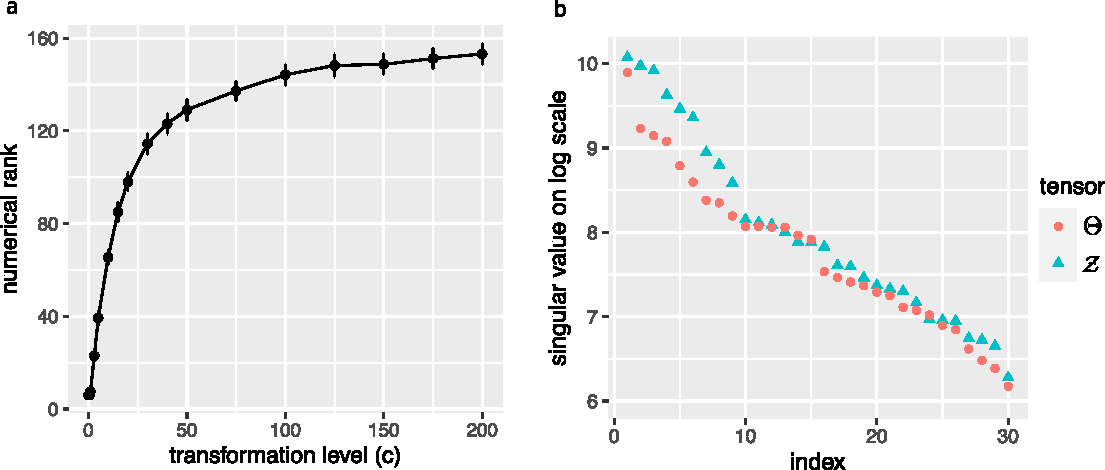
\includegraphics[width=.47\textwidth]{figure/example_comb.pdf}
\caption{(a) Numerical rank of $\Theta=f(\tZ)$ versus $c$ in Example 1. (b) Top $d=30$ tensor singular values in Example 2. }\label{fig:example}
\end{figure}

\begin{figure*}[h!]
\vspace{-.2cm}
\centerline{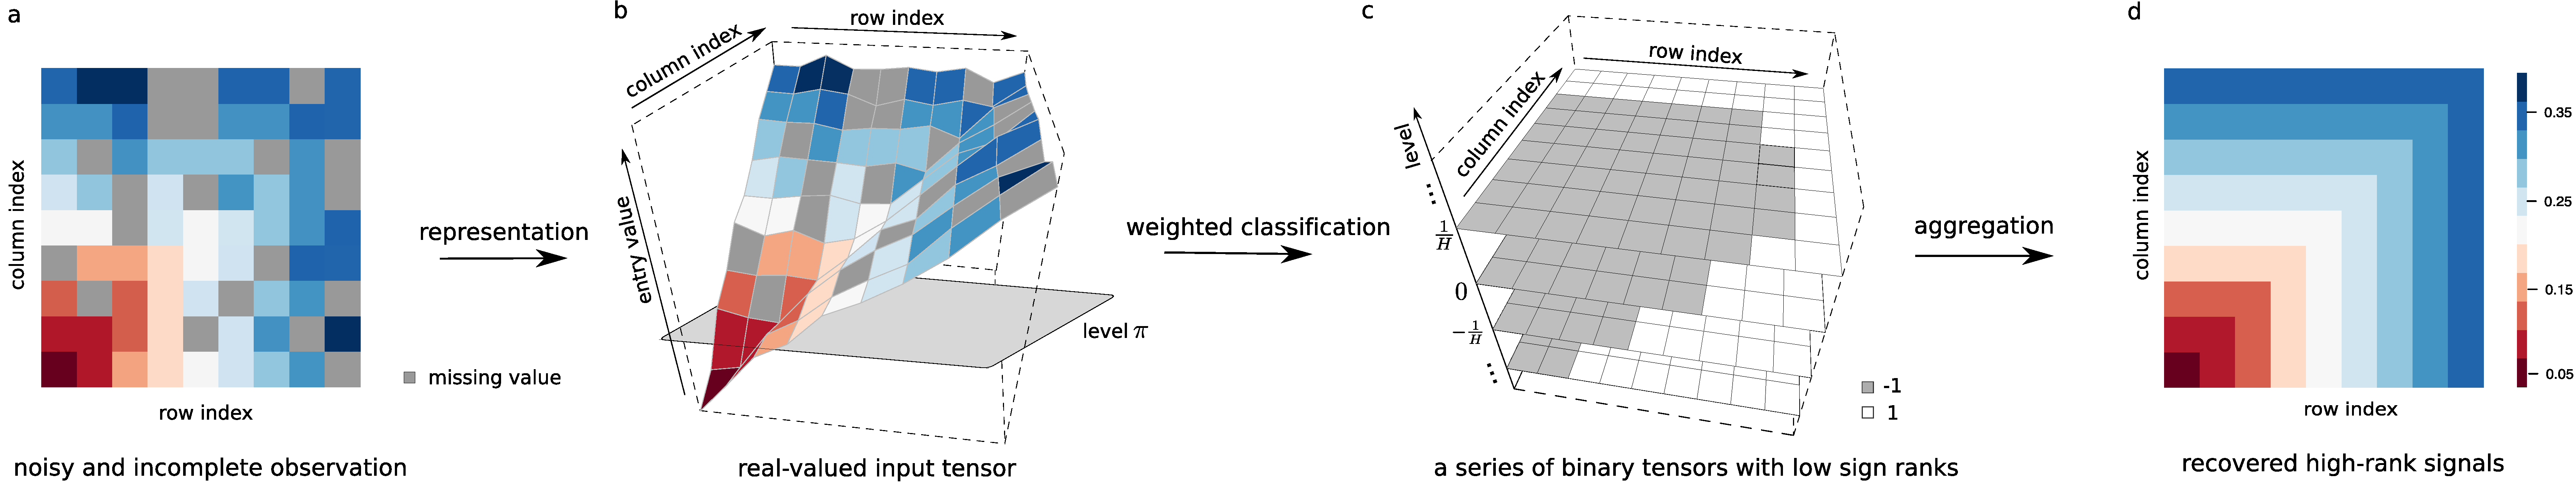
\includegraphics[width=1\textwidth]{figure/image_new2.pdf}}
\caption{Illustration of our proposed method. For visualization purpose, we plot an order-2 tensor (a.k.a. matrix) in the figure; similar procedure applies to higher-order tensors. (a): input tensor $\tY_\Omega$ with noisy and incomplete entries. (b) and (c): our method uses weighted classification to estimate sign tensors $\sign(\Theta-\pi)$ for a sequence of levels $\pi\in \{-1,\ldots,-{1\over H},0,{1\over H},\ldots,1\}$. (d) output tensor $\hat \Theta$ with denoised and imputed entries. The depicted example is based on Example 5, where the true signal matrix has full rank. }\label{fig:demo}
\end{figure*}

The first example reveals the sensitivity of tensor rank to order-preserving transformations. Let $\tZ \in \mathbb{R}^{30\times 30\times 30}$ be an order-3 tensor with $\text{rank}(\tZ)=3$. Suppose a monotonic transformation $f(z)=(1+\exp(-cz))^{-1}$ is applied to $\tZ$ entrywise, and we observe data from model~\eqref{eq:model} with the signal tensor $\Theta=f(\tZ)$. Figure~\ref{fig:example}(a) plots the numerical rank of $\Theta$ versus $c$. %Note that a smaller $c$ implies an approximate linear transformation $f(z)\approx -cz$, whereas a larger $c$ implies a higher nonlinearity $z\mapsto \{0,1\}$. 
As we see, the rank increases rapidly with $c$, rending traditional low-rank tensor methods ineffective even in the presence of mild order-preserving nonlinearities. In applications of digital processing~\cite{karbasi2012robust} and genomics analysis~\cite{wang2019three}, the tensor of interest often undergoes some unknown transformation prior to measurements. The sensitivity to transformation therefore makes the low-rank model less desirable in practice. 


The second example shows that the classical low-rankness may exclude important specially-structured tensors. Here we consider the signal tensor of the form $\Theta=\log(1+\tZ)$, where $\tZ$ is an order-3 tensor with entries $\tZ(i,j,k)={1\over d}\max(i,j,k)$ for $(i,j,k)\in[d]^3$. The matrix analogy of this $\Theta$ was studied in~\citet{chan2014consistent} in the context of graphon analysis. In this case neither $\Theta$ nor $\tZ$ is low-rank; indeed, both tensors have rank lower bounded by dimension $d$ as illustrated in Figure~\ref{fig:example}(b). However, classical low-rank models fail to address these types of structures. 

In the above and many other examples, the signal tensors $\Theta$ of interest are of high rank. These structures are hardly detectable using classical low-rank models. New methods that allow flexible tensor modeling have yet to be developed. 


\subsection{Our proposal and contribution}\label{sec:overview}
We briefly provide the intuition of our method and summarize the contributions. In the earlier two high-rank examples, if we examine the sign of the $\pi$-shifted signal, $\sign(\Theta-\pi)$ for any given $\pi$, then these sign tensors exhibit easily detectable low-rankness. In particular, the signal tensor in example 1 has the same sign pattern as a rank-$4$ tensor, since $\sign(\Theta-\pi)=\sign(\tZ-f^{-1}(\pi))$. The signal tensor in example 2 has the same sign pattern as a rank-2 tensor, since $\sign(\Theta-\pi)=\sign(\max(i,j,k)-d(e^{\pi}-1))$.


The above observation suggests a general framework to analyze both low- and high-rank signal tensors. Figure~\ref{fig:demo} illustrates the main crux of our method. We dichotomize the data tensor into a series of sign tensors, $\sign (\tY_\Omega-\pi)$, for $\pi\in \tH=\{-1,\ldots, {\scriptstyle -{1\over H}},0,{\scriptstyle {1\over H}},\ldots,1\}$, and then estimate the sign signals, $\sign(\Theta-\pi)$, by performing classification
\[
\hat \tZ_\pi=\argmin_{\text{low rank tensor $\tZ$}} L(\sign(\tZ),\ \sign (\tY_\Omega-\pi)).
\]
Here, $L(\cdot,\cdot)$ denotes a carefully-designed classification objective function which will be described in later sections. The final proposed tensor estimate is 
\[
\hat \Theta = {1\over 2H+1}\sum_{\pi \in \tH} \sign(\hat \tZ_\pi).
\]
Our approach is built on the nonparametric sign representation of signal tensors, and the estimate $\hat \Theta$ is essentially estimated from dichotomized tensor series $\{\sign(\tY_\Omega-\pi)\colon \pi \in \tH\}$. Surprisingly, we show that proper analysis based on dichotomized data not only preserves all information in the original signals, but also brings benefits of accuracy and flexibility over classical low-rank models. The method enjoys both statistical effectiveness and computational efficiency. 

 Our method features several advantages. In contrast to earlier methods~\cite{hong2020generalized,filipovic2015tucker}, our method recover the signal tensor under a wide range of low- and high-rank tensor models. Our method brings the nonparametric advantages of flexibility into tensor estimation and completion. The algorithm achieves computational efficiency by leveraging classification and divide-and-conquer algorithms.


\subsection{Preliminaries}
We use the shorthand $[n]$ to denote the $n$-set $\{1,\ldots,n\}$ for $n\in\mathbb{N}_{+}$. We use $\otimes$ to denote the outer product of vectors, $\vnormSize{}{\mx}$ to denote the vector $2$-norm, and $\mathbf{S}^{d-1}=\{\mx\in\mathbb{R}^d\colon \vnormSize{}{\mx}=1\}$ to denote the $(d-1)$-dimensional unit sphere. Let $\tY\in\mathbb{R}^{d_1\times \cdots \times d_K}$ denote an order-$K$ $(d_1,\ldots,d_k)$-dimensional tensor, and $\tY(\omega)\in\mathbb{R}$ denote the tensor entry indexed by $\omega \in[d_1]\times \cdots \times [d_K]$. The Frobenius norm of $\tY$ is defined as $\FnormSize{}{\tY}=\sqrt{\sum_{\omega}\tY^2(\omega)}$. Unlike matrices, various notions of decomposition have been developed for tensors of order $K\geq 3$. The Canonical Polyadic (CP) tensor decomposition~\cite{hitchcock1927expression} for a tensor $\Theta\in\mathbb{R}^{d_1\times \cdots \times d_K}$ is defined as
\begin{equation}\label{eq:CP}
\Theta=\sum_{s=1}^r\lambda_s \ma^{(1)}_s\otimes\cdots\otimes \ma^{(K)}_s,
\end{equation}
where $\lambda_1\geq \cdots \geq \lambda_r>0$ are called tensor singular values, and $\ma^{(k)}_s \in \mathbf{S}^{d_k-1}$ are called tensor singular vectors, for all $s\in[r]$, $k\in[K]$. The minimal $r$ for which the decomposition~\eqref{eq:CP} holds is called the tensor rank, denoted as $\rank(\Theta)$. 

We use $\sign(\cdot)\colon \mathbb{R}\to\{-1,1\}$ to denote the sign function, where $\sign(y)=1$ if $y\geq 0$ and $-1$ otherwise. We allow univariate functions, such as $\sign(\cdot)$ or general $f\colon \mathbb{R}\to\mathbb{R}$, to be applied to tensors in an element-wise manner. 
%For a tensor $\Theta\in\mathbb{R}^{d_1\times \cdots \times d_K}$, its sign pattern $\sign(\Theta)$ is an order-$K$ $(d_1,\ldots,d_K)$-dimensional binary tensor with entries in $\{-1,1\}$. 



\section{Observation model}

Let $\tY$ be an order-$K$ $(d_1,\ldots,d_K)$-dimensional data tensor. Assume that $\tY$ is generated from the following model,
\begin{equation}\label{eq:model}
\tY=\Theta+\tE,
\end{equation}
where $\Theta\in\mathbb{R}^{d_1\times \cdots \times d_K}$ is the unknown signal tensor of interest, and $\tE$ is a noise tensor consisting of mean-zero, independent but not necessarily identically distributed entries. We allow heterogenous noise in that the marginal distribution of noise entry $\tE(\omega)$ may depend on $\omega$. In general, we allow $\tY(\omega)$ to take either continuous or discrete value in a bounded interval $[-A, A]$, where $A>0$. Unless otherwise specified, we assume $A=1$ throughout the paper. 

Our observation is an incomplete data tensor from~\eqref{eq:model}, denoted $\tY_\Omega$, where $\Omega\subset[d_1]\times\cdots\times[d_K]$ is the index set of observed entries. We consider a general model on $\Omega$ that allows both uniform and non-uniform samplings. Specifically, let $\Pi=\{\pi_\omega\}$ be an arbitrarily predefined probability distribution over the full index set with $\sum_{\omega\in[d_1]\times \cdots \times [d_K]}\pi_\omega=1$. We assume the entries $\omega$ in $\Omega$ are i.i.d.\ draws with replacement from the full index set using distribution $\Pi$. The sampling rule will be denoted as $\omega\sim \Pi$.


\section{Sign representable tensors}\label{sec:representation}
In this section, we develop sign representable tensor models for $\Theta$ in~\eqref{eq:model}. The algebraic and statistical characterization of sign tensor series provides the accuracy guarantee for our method. 

\subsection{Sign-rank and sign tensor series}\label{sec:sign-rank}
Let $\Theta$ be a continuous-valued tensor, and $\sign (\Theta)$ be the corresponding sign patten. The sign pattern induces an equivalence relationship between tensors. Two tensors are called sign equivalent, denoted $\simeq$, if they share the same sign patterns. 

\begin{defn}[Sign-rank]
The sign-rank of a tensor $\Theta\in\mathbb{R}^{d_1\times \cdots \times d_L}$ is the minimal rank among all tensors that share the same sign patterns as $\Theta$; i.e.,
\[
\srank(\Theta) = \min \{\rank(\Theta')\colon  \Theta'\simeq \Theta,\ \Theta'\in\mathbb{R}^{d_1\times \cdots \times d_K}\}.
\]
\end{defn}
The sign-rank is also called \emph{support rank}~\cite{cohn2013fast}, \emph{minimal rank}~\cite{alon2016sign}, and \emph{nondeterministic rank}~\cite{de2003nondeterministic} in the filed of combinatorics and information theory. Earlier work defines sign-rank for binary tensors/matrices only; we extend the notion to continuous-valued tensors. Note that the sign-rank concerns only the sign pattern but discards the magnitudes information of $\Theta$. In particular, $\srank(\Theta)=\srank(\sign \Theta)$. 

Like most tensor problems~\cite{hillar2013most}, determining the sign-rank for a general tensor is NP hard~\cite{alon2016sign}. Fortunately, tensors arisen in application often possess special structures that facilitate analysis. We show that the family of low sign-rank tensors is strictly broader than usual low-rank tensors. This is because sign-rank is upper bounded by the usual rank. More generally, 
\begin{prop}[Upper bounds of sign-rank]~\label{cor:monotonic} For any monotonic function $g\colon \mathbb{R}\to \mathbb{R}$ with $g(0)=0$, 
\[
\textup{srank}(\Theta)\leq\rank(g(\Theta)).
\]
\end{prop}
Conversely, the sign-rank can be dramatically smaller than the usual rank, as we have shown in Section~\ref{sec:example}.
\begin{prop}[Broadness]\label{prop:extention}For every order $K\geq 2$ and dimension $d$, there exist order-$K$ $(d,\ldots,d)$-dimensional tensors $\Theta$ such that $\rank(\Theta)=d$ and $\srank(\Theta)=2$.
\end{prop}
Several common examples are provided in Appendix, in which we show the tensor rank grows with dimension $d$ but the sign-rank remains a constant. The results highlight the advantages of using sign-rank in the high-dimensional tensor analysis. Corollary~\ref{cor:monotonic} and Proposition~\ref{prop:extention} together demonstrate the strict broadness of low sign-rank tensor family over the usual low-rank tensor family. 

We now introduce a tensor family, which we coin as ``sign representable tensors'', for the signal tensors in model~\eqref{eq:model}. 
\begin{defn}[Sign representable tensors] 
Fix a level $\pi\in[-1,1]$. A tensor $\Theta$ is called $(r,\pi)$-sign representable, if the tensor $(\Theta-\pi)$ has sign-rank bounded by $r$. A tensor $\Theta$ is called $r$-sign (globally) representable, if $\Theta$ is $(r,\pi)$-sign representable for all $\pi\in[-1,1]$. The collection $\{\sign(\Theta-\pi)\colon \pi \in[-1,1]\}$ is called the sign tensor series. 
We use $\caliP(r)=\{\Theta\colon \srank(\Theta-\pi)\leq r \text{ for all }\pi\in[-1,1]\}$ to denote the $r$-sign representable tensor family.
\end{defn}
We show that the $r$-sign representable tensor family is a general model that incorporates most existing tensor models, including low-rank tensors, single index models, GLM models, and certain hypergraphon models. 

\begin{example}[CP/Tucker low-rank models] The CP and Tucker low-rank models are the two most popular tensor models~\cite{anandkumar2014tensor,montanari2018spectral,kadmon2018statistical,cai2019nonconvex}. Let $\Theta$ be a low-rank tensor with CP rank $r$. We see that $\Theta$ belongs to the sign representable family, i.e., $\Theta\in\caliP(r+1)$ (the constant $1$ is due to $\rank(\Theta-\pi)\leq r+1$). Similarly, Tucker low-rank tensors $\Theta\in\caliP(r+1)$, where $r=\prod_kr_k$ with $r_k$ being the $k$-th mode Tucker rank of $\Theta$.  
\end{example} 

\begin{example}[Tensor block models (TBMs)] Tensor block model~\cite{wang2019multiway,chi2020provable} assumes a checkerbord structure among tensor entries under marginal index permutation. The signal tensor $\Theta$ takes at most $r$ distinct values, where $r$ is the total number of multiway blocks. Our model incorporates TBM because $\Theta \in \caliP(r)$. 
\end{example}


\begin{example}[Generalized linear models (GLMs)] Let $\tY$ be a binary tensor from a tensor logistic model~\cite{wang2018learning} with mean $\Theta=\mathbb{E}(\tY)=\text{logit}(\tZ)$, where $\tZ$ is a latent low-rank tensor. By definition, $\Theta$ is a low-rank sign representable tensor, although the usual rank of $\Theta$ is often high (see Section~\ref{sec:example}). Same conclusion holds for general exponential-family tensors with a (known) link function~\cite{hong2020generalized}. 
\end{example}

\begin{example}[Single index models (SIMs)] Single index model is a flexible semiparametric model initially proposed in economics~\cite{robinson1988root} and has recently been popular in high-dimensional statistics~\cite{balabdaoui2019least,ganti2017learning,alquier2013sparse}. We here extend the model to high-dimensional tensors $\Theta$. The SIM assumes the existence of a (unknown) monotonic function $g\colon \mathbb{R}\to \mathbb{R}$ such that $g(\Theta)$ has rank $r$. We see that $\Theta$ belongs to the sign representable family; i.e., $\Theta\in \caliP(r+1)$. 
\end{example}

\begin{example}[Min/Max hypergraphon] Graphon is a popular nonparametric model for networks~\cite{chan2014consistent,xu2018rates}, and we have extended the model for tensors in Section~\ref{sec:example}. Here we revisit the model for generality. Let $\Theta$ be an order-$K$ tensor generated from the hypergraphon $\Theta(i_1,\ldots,i_K)=\log(1+\max_kx^{(k)}_{i_k})$, where $x^{(k)}_{i_k}\sim \text{Unif}[0,1]$ i.i.d.\ for all $i_k\in[d_k]$ and $k\in[K]$. Every sign tensor $\sign(\Theta-\pi)$ in the series of $\pi\in[0,\ \log 2]$ is a block tensor with at most two blocks, so $\Theta \in \caliP(2)$. 

The results extend to general min/max hypergraphons. Let $g(\cdot)$ be a continuous univariate function with at most $r\geq 1$ real-valued roots in the equation $g(z)=\pi$; this property holds, e.g., when $g(z)$ is a polynomial of degree $r$. Then, the tensor $\Theta$ generated from $\Theta(i_1,\ldots,i_K)=g(\max_kx^{(k)}_{i_k})$ belongs to $\caliP(r+1)$. Same conclusion applies if the maximum is replaced by minimum.
\end{example}

\subsection{Statistical characterization of sign tensors via weighted classification}\label{sec:identifiability}

Accurate estimation of a sign representable tensor crucially depends on the behavior of sign tensor series $\sign(\Theta-\pi)$. In this section, we show that weighted classification completely characterizes the sign tensors. The results bridge the algebraic and statistical properties of sign representable tensors, thereby providing the theoretical guarantee for our nonparametric algorithm (Figure~\ref{fig:demo}).
 
For a given $\pi \in [-1,1]$, define a $\pi$-shifted data tensor $\bar \tY_\Omega$ with entries $\bar \tY(\omega) = (\tY(\omega)-\pi)$ for all $\omega\in \Omega$. We propose a weighted classification objective
\begin{equation}\label{eq:sample}
L(\tZ, \bar \tY_\Omega)= {1\over |\Omega|}\sum_{\omega \in \Omega}\KeepStyleUnderBrace{|\bar \tY(\omega)|}_{\text{entry-specific weight}} \times \KeepStyleUnderBrace{| \sign \tZ(\omega)-\sign \bar \tY(\omega)|}_{\text{classification loss}},
\end{equation}
where $\tZ\in\mathbb{R}^{d_1\times \cdots \times d_K}$ is the decision variable to be optimized, $|\bar \tY(\omega)|$ is the entry-specific weight equal to the distance from the tensor entry to the target level $\pi$. The objective reduces to usual classification loss in the special case when the data tensor is binary and the target level $\pi=0$.

Our proposed entry-specific weight is important for characterizing $\sign(\Theta-\pi)$, as we show now. Define the weighted classification risk 
\begin{equation}\label{eq:population}
\textup{Risk}(\tZ)=\mathbb{E}_{\tY_\Omega}L(\tZ,\bar\tY_\Omega),
\end{equation}
where the expectation is taken with respect to $\tY_\Omega$ under model~\eqref{eq:model} and the sampling distribution $\omega\sim\Pi$. Note that the form of $\textup{Risk}(\cdot)$ implicitly depends on $\pi$; we suppress $\pi$ when no confusion arises. 
\begin{prop}[Global optimum of weighted risk]\label{prop:global}
Suppose the data $\tY_\Omega$ is generated from model~\eqref{eq:model} with $\Theta \in \caliP(r)$. Then, for all $\bar \Theta$ that are sign equivalent to $\sign(\Theta-\pi)$, 
\begin{align}\label{eq:optimal}
\textup{Risk}(\bar \Theta )&=\inf\{\textup{Risk}(\tZ)\colon \tZ\in\mathbb{R}^{d_1\times \cdots \times d_K}\},\notag \\
&=\inf\{\textup{Risk}(\tZ)\colon \textup{rank} \tZ\leq r\}.
\end{align}
\end{prop}
The results show that the sign tensor $\sign(\Theta-\pi)$ optimizes the weighted classification risk. This fact suggests a practical procedure to estimate $\sign(\Theta-\pi)$ via optimizing the empirical risk $L(\tZ,\bar \tY_\Omega)$. The entry-specific weight incorporates the magnitude information in the classification, where entries far away from the target level are penalized more heavily in the objective. 

In order to establish the recovery guarantee, we address the uniqueness (up to sign equivalence) of the optimizer for $\risk(\cdot)$. Essentially, this is a converse problem of Proposition~\ref{prop:global} asking whether optimizing $\risk(\cdot)$ is sufficient for recovering $\sign(\Theta-\pi)$. The local behavior of $\Theta$ around $\pi$ turn out to play a key role in the accuracy guarantee. 

Some additional notation is needed. %Recall that $\omega\sim \Pi$ denotes the sampling distribution over tensor indices. 
We use $\tN=\{\pi\colon$  $\mathbb{P}_{\omega\sim \Pi}(\Theta(\omega)=\pi)\neq 0\}$ to denote the set of mass points of $\Theta$ under $\Pi$. Assume there exists a constant $C>0$, independent of tensor dimension, such that $|\tN|\leq C$. Note that both $\Pi$ and $\Theta$ implicitly depend on the tensor dimension. Our assumptions are imposed to $\Pi=\Pi(d)$ and $\Theta=\Theta(d)$ in the high-dimensional regime uniformly as $d:=\min_kd_k\to\infty$. 

%Unless otherwise stated, all relevant assumptions should be interpreted as uniform conditions for all large $d$. 

\begin{assumption}[$\alpha$-smoothness]\label{ass:margin} 
Fix $\pi\notin \tN$. Assume there exist constants $\alpha=\alpha(\pi)\geq 0, c=c(\pi) >0$, independent of tensor dimension, such that, 
\begin{equation}\label{eq:smooth}
\sup_{0\leq t<\rho(\pi, \tN)}{\mathbb{P}_{\omega \sim \Pi}[\omega \colon |\Theta (\omega)-\pi|\leq t ]\over t^\alpha} \leq c,
\end{equation}
where $\rho(\pi,\tN):=\min_{\pi'\in \tN}|\pi-\pi'|$ denotes the distance from $\pi$ to the nearest point in $\tN$. The largest possible $\alpha=\alpha(\pi)$ is called the smoothness index at level $\pi$. We make the convention that $\alpha= \infty$ if the set $\{\omega\colon |\Theta(\omega)-\pi|\leq t\}$ has zero measure, implying few entries of $\Theta$ around the level $\pi$. We call the tensor $\Theta$ is $\alpha$-globally smooth, if~\eqref{eq:smooth} holds with a global constant $c>0$ for all $\pi\in[-1,1]$ except for a finite number of levels. 
\end{assumption}

The smoothness index $\alpha$ quantifies the intrinsic hardness of recovering $\sign(\Theta-\pi)$ from $\risk(\cdot)$. The value of $\alpha$ depends on both the sampling distribution $\omega\sim \Pi$ and the behavior of $\Theta(\omega)$. The recovery is more difficult at levels where the point mass concentrates (small $\alpha$). A large value of $\alpha>1$ corresponds a plateau-type zero density of $\Theta(\omega)$ around $\pi$, or equivalently, when the cumulative distribution function (CDF) $F(\pi):=\mathbb{P}_{\omega\sim \Pi}[\Theta(\omega)\leq \pi]$ remains flat around $\pi$. A small value of $\alpha<1$ indicates the nonexistent (infinite) density at level $\pi$, or equivalently, when the CDF jumps at $\pi$.  A typical case is $\alpha=1$ when the CDF has finite non-zero derivative in the vicinity of $\pi$. Table~\ref{tab:simulation} illustrates the CDFs for various common models; the details will be described in Simulation section. 
%{\color{red}Conjecture: If the global smoothness index $\alpha>1$, then $\tN\geq 1$. }


We now reach the main theorem in this section. For two tensors $\Theta_1,\Theta_2$, define the mean absolute error (MAE)
\[
\text{MAE}(\Theta_1, \Theta_2)\stackrel{\text{def}}{=}\mathbb{E}_{\omega\sim \Pi}\onenormSize{}{\Theta_1-\Theta_2}.
\]
\begin{thm}[Identifiability]\label{thm:population}Under Assumption~\ref{ass:margin}, for all tensors $\bar \Theta \simeq \sign(\Theta-\pi)$ and tensors $\tZ\in\mathbb{R}^{d_1\times \cdots \times d_K}$,
\[
\textup{MAE}(\sign \tZ, \sign \bar \Theta) \leq C(\pi)\left[\textup{Risk}(\tZ)-\textup{Risk}( \bar \Theta)\right]^{\alpha/(\alpha+1)},
\]
where $C(\pi)>0$ is independent of $\tZ$. 
\end{thm}
The result establishes the stability of recovering sign tensors $\sign (\Theta-\pi)$ from optimizing the population risk~\eqref{eq:population}. Furthermore, the bound immediately suggests the uniqueness of the optimizer for $\text{Risk}(\cdot)$ up to a zero-measure set under $\Pi$, as long as $\alpha\neq 0$. We find that a higher value of $\alpha$ implies more stable recovery. Similar results hold for the empirical risk minimization~\eqref{eq:sample} (see Section~\ref{sec:estimation} for details). 

We conclude this section by relating Assumption~\ref{ass:margin} to the examples described in Section~\ref{sec:sign-rank}. For simplicity, suppose $\Pi$ is the uniform sampling for now. Based on definition, the tensor block model is $\infty$-globally smooth. This is because there are finitely many elements in $\tN$, i.e, the set of distinct block means in $\Theta$. Furthermore, we have $\alpha= \infty$ for all $\pi \notin \tN$, since the numerator in~\eqref{eq:smooth} is zero for all such $\pi$. The min/max hypergaphon with a $r$-degree polynomial function is $1$-globally smooth, because $\alpha=1$ for all $\pi$ in the function range except at most $(r-1)$ many (stationary) levels. 


\section{Nonparametric tensor completion via sign series}\label{sec:estimation}
In previous sections we have established the sign representation and sign series recovery for the signal tensor. In this section, we present our algorithm proposed in Section~\ref{sec:overview} (Figure~\ref{fig:demo}) in details. We provide the estimation error bound and address the empirical implementation of the algorithm. 

\subsection{Estimation error and sample complexity}

Given a noisy incomplete tensor observation $\tY_\Omega$ from model~\eqref{eq:model}, we cast the problem of estimating $\Theta$ into a series of weighted classifications. Specifically we propose a tensor estimator using the sign representation,
\begin{equation}\label{eq:est}
\hat \Theta = {1\over 2H+1}\sum_{\pi \in \tH}\sign{\hat \tZ_\pi},
\end{equation}
where $\hat \tZ_\pi\in\mathbb{R}^{d_1\times \dots\times d_K}$ is the $\pi$-weighted classifier estimated at levels $\pi \in \tH=\{-1,\ldots,-{1\over H}, 0, {1\over H},\ldots,1\}$,
\begin{equation}\label{eq:estimate}
\hat \tZ_\pi = \argmin_{\tZ\colon \text{rank}\tZ\leq r} L(\tZ, \sign(\tY_\Omega-\pi)).
\end{equation}
Here $L(\cdot,\cdot)$ denotes the weighted classification objective defined in~\eqref{eq:sample}, where we have plugged $\bar \tY_\Omega=(\tY_\Omega-\pi)$ in the expression, and the rank constraint follows from Proposition~\ref{prop:global}. For the theory, we assume the true $r$ is known; in practice, $r$ could be chosen in a data adaptive fashion via cross-validation or elbow method~\cite{hastie2009elements}. Figure~\ref{fig:demo} illustrates the main steps in our proposed estimation. 

The next theorem establishes the statistical convergence for the sign tensor estimation~\eqref{eq:estimate}, which is an important ingredient for the signal tensor estimator $\hat \Theta$ in~\eqref{eq:est}. 

 \begin{thm}[Sign tensor errors]\label{thm:classification} Suppose $\Theta\in\caliP(r)$ and $\Theta(\omega)$ is $\alpha$-globally smooth under $\omega\sim \Pi$, where $\alpha\in(0,1]$. Let $\hat \tZ_\pi$ be the estimator in~\eqref{eq:estimate}, and denote $d_{\max}=\max_{k\in[K]} d_k$. Then, for all $\pi\in[-1,1]$ except for a finite number of levels, with very high probability over $\tY_\Omega$, 
\begin{align}\label{eq:bound}
\textup{MAE}(\sign \hat \tZ_\pi, \sign(\Theta-\pi)) \lesssim & \left({d_{\max} r \over |\Omega|}\right)^{\alpha\over \alpha+2}\notag \\
&+{1 \over \rho^2(\pi, \tN)} {d_{\max}r \over |\Omega|}.
\end{align}
\end{thm}
Theorem~\ref{thm:classification} provides the error bound for the estimated sign tensors. Compared to the population version results in Theorem~\ref{thm:population}, we here explicitly reveal the dependence of accuracy on the sample complexity and on the level $\pi$. The result~\eqref{eq:bound} shows the sign error decreases with $|\Omega|$, provided that $\alpha \neq 0$. In particular, our sign estimate achieves consistent recovery using as few as $\tilde O(d_{\max}r)$ noisy observations. 
%In the case of equal dimension and full observation $|\Omega|=d^K$, the sign estimate reaches a fast rate $d^{-(K-1)}$ when $\alpha=\infty$. 

\begin{figure*}[h]
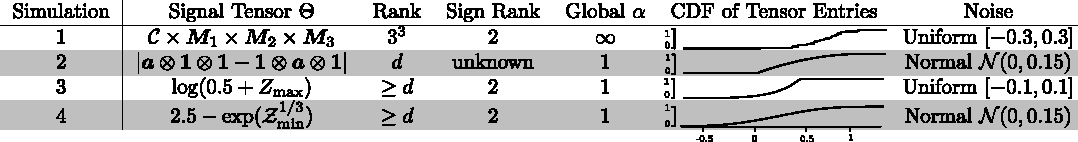
\includegraphics[width=1\textwidth]{figure/simulation_new.pdf}
\vspace{-.8cm}
\caption{Simulation models used for comparison. We use $\mM_k\in\{0,1\}^{d\times 3}$ to denote membership matrices, $\tC\in\mathbb{R}^{3\times 3\times 3}$ the block means, $\ma={1\over d}(1,2,\ldots,d)^T \in\mathbb{R}^d$, $\tZ_{\max}$ and $\tZ_{\min}$ are order-3 tensors with entries ${1\over d}\max(i,j,k)$ and ${1\over d}\min(i,j,k)$ respectively.}\label{tab:simulation}
\vspace{-.4cm}
\end{figure*}


Combining the sign representability of the signal tensor and the sign estimation accuracy, we obtain the main results on our nonparametric tensor estimation method.
\begin{thm}[Tensor estimation error]\label{thm:estimation} Consider the same conditions of Theorem~\ref{thm:classification}. Let $\hat \Theta$ be the estimate in~\eqref{eq:est}. With very high probability over $\tY_\Omega$,
\begin{equation}\label{eq:bound}
\textup{MAE}(\hat \Theta, \Theta)\lesssim \left({d_{\max} r \over |\Omega|}\right)^{\alpha/(\alpha+2)}+{1\over H}+H{d_{\max} r \over |\Omega|}.
\end{equation}
In particular, setting $\scriptstyle H\asymp \left( |\Omega|\over d_{\max}r\right)^{1/2}$ yields the error bound
\begin{equation}\label{eq:real}
\textup{MAE}(\hat \Theta, \Theta)\lesssim \left(d_{\max}r \over|\Omega|\right)^{{\alpha \over \alpha+2} \vee {1\over 2}}.
\end{equation}
\end{thm}
Theorem~\ref{thm:estimation} demonstrates the convergence rate of our tensor estimation. The bound~\eqref{eq:bound} reveals three sources of errors: the estimation error inherited from sign tensors, the bias from sign series representations, and the variance thereof. The resolution parameter $H$ controls the bias-variance tradeoff. We remark that the signal estimation error~\eqref{eq:real} is generally no better than the corresponding sign error~\eqref{eq:bound}. This is to be expected, since magnitude estimation is a harder problem than sign estimation. 

In the special case of full observation with equal dimension $d_1=\cdots=d_K=d$, our signal estimate achieves convergence rate
\begin{equation}
\textup{MAE}(\hat \Theta, \Theta)\leq \left(r\over d^{K-1}\right)^{{\alpha \over \alpha+2} \vee {1\over 2}}.
\end{equation}
In contrast to earlier methods, our estimation accuracy applies to both low- and high-rank signal tensors $\Theta$. The rate depends on the sign complexity $\Theta\in\caliP(r)$, and this $r$ is often much smaller than the usual tensor rank (see Section~\ref{sec:sign-rank}). Therefore, our method not only incorporates the earlier work on low-rank tensor estimation but also addresses a broad family that was previously impossible. 

We apply our method to selected examples in Section~\ref{sec:sign-rank}, and compare the results with existing literature. The numerical comparison is provided in Section~\ref{sec:simulation}. 
\begin{customexample}{2}[Tensor block models]
Consider a tensor block model with $r$ multiway blocks in total. Our result implies a rate $\tO(d^{-(K-1)/2})$ by taking $\alpha=\infty$. This rate agrees with the  previous root-mean-square error (RMSE) for block tensor estimation~\cite{wang2019multiway}.
\end{customexample}

\begin{customexample}{3} [CP/Tucker and GLMs] 
Consider a GLM tensor $\Theta=g(\tZ)$, where $g$ is a known link function and $\tZ$ is a latent low-rank tensor. Suppose the marginal density of $\Theta(\omega)$ is bounded from above. Applying our results with $\alpha=1$ yields $\tO(d^{-(K-1)/3})$. Note that this rate is slightly slower than the parametric RMSE rate~\cite{zhang2018tensor,wang2018learning}. One possible reason is that our result remains valid for unknown $g$ and more general high-rank tensors with $\alpha=1$. The tensor family involved in our upper bound is broader than parametric models. 
\end{customexample}

The following sample complexity for nonparamtric tensor completion is an immediate corollary of Theorem~\ref{thm:estimation}. 
\begin{cor}[Sample complexity for nonparametric completion] Under the same conditions of Theorem~\ref{thm:estimation}, with very high probability over $\tY_\Omega$, 
\[
\textup{MAE}(\hat \Theta, \Theta)\to 0, \quad \text{as}\quad {|\Omega|\over {d_{\max}} r}\to \infty.
\]
\end{cor}
Our result improves earlier work~\cite{ghadermarzy2019near,cai2019nonconvex} by allowing both low- and high-rank signals. Note that $\tilde \tO(d_{\max}r)$ roughly matches the degree of freedom in sign tensor series, suggesting the optimality of our sample requirement. 

\subsection{Numerical implementation}
This section addresses the practical implementation of our estimation~\eqref{eq:est} illustrated in Figure~\ref{fig:demo}. Our sign representation of tensor estimate $\Theta$ is a simple average of $H$ sign tensors, which can be solved in a divide-and-conquer fashion. Briefly, we estimate the sign tensors $\tZ_\pi$ (which are detailed in the next paragraph) for the series $\pi \in \tH$ through parallel implementation, and then aggregate the results for the final output. This approach maintains low computational cost similar to a single sign tensor estimation.  

\begin{figure*}[h!]
\vspace{-.4cm}
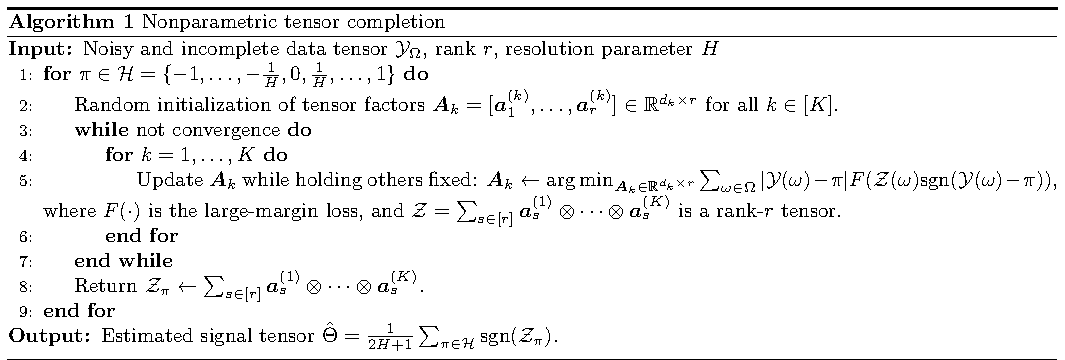
\includegraphics[width=\textwidth]{figure/algorithm.pdf}
\vspace{-.8cm}
\end{figure*}


For the sign tensor estimation~\eqref{eq:estimate}, the problem reduces to binary tensor decomposition with a weighted classification loss. A number of algorithms have been developed for this problem~\cite{ghadermarzy2018learning,wang2018learning,hong2020generalized}. We adopt similar ideas by tailoring to our contexts. Following the common practice in classification, we replace the binary loss $\ell(z,y)=|\sign z - \sign y|$ with a surrogate loss $F(m)$ as a continuous function of margin $m\stackrel{\text{def}}{=}z\sign(y)$. Examples of large-margin loss are hinge loss $F(m) = (1-m)_+$ for support vector machines, logistic loss $F(m) =\log(1+e^{-m})$ for important vector machines, and nonconvex $\psi$-loss $F(m)=2\min(1,(1-m)_+)$ with $m_{+}=\max(m,0)$. We implement the hinge loss and logistic loss in our algorithm, although our framework is applicable to general large-margin losses~\citep{bartlett2006convexity}. 


The rank constraints in the optimization~\eqref{eq:est} have been extensively studied in literature. Recent developments involve convex norm relaxation~\cite{ghadermarzy2018learning} and nonconvex optimization~\cite{wang2018learning, han2020optimal}. Unlike matrices, computing the tensor convex norm is NP hard, so we choose (non-convex) alternating optimization due to its numerical efficiency. Briefly, we use the rank decomposition~\eqref{eq:CP} of $\tZ=\tZ(\mA_1,\ldots, \mA_K)$ 
%\mA_K)=\sum_{s=1}^r\ma^{(1)}_s\otimes \cdots \otimes \ma^{(K)}_s$ write the optimization~\eqref{eq:estimate} as
%\begin{align}
%\min_{\mA_k\colon k\in[K]}&\sum_{\omega\in \Omega}|\tY-\pi|F(\tZ(\omega)\sign(\tY(\omega)-\pi)),\\
%\text{subject to }\tZ&=\tZ(\mA_1,\ldots,\mA_K)=\sum_{s=1}^r\ma^{(1)}_s\otimes \cdots \otimes \ma^{(K)}_s,
%\end{align}
where $\mA_k=[\ma^{(k)}_1,\ldots,\ma^{(k)}_r]\in\mathbb{R}^{d_k\times r}$ are unknown factor matrices to optimize. We numerically solve \eqref{eq:est} by optimizing one factor $\mA_k$ at a time while holding others fixed, and iterate until convergence. Each suboptimization reduces to a convex optimization with a low-dimensional decision variable. Following common practice in tensor optimization~\cite{anandkumar2014tensor,hong2020generalized}, we run the optimization from multiple initializations to locate a final estimate with the lowest objective value. The full procedure is described in Algorithm 1.


\section{Simulation}\label{sec:simulation}
In this section, we compare our nonparametric tensor method ({\bf NonParaT}) with two alternative approaches: low-rank tensor CP decomposition ({\bf CPT}), and the matrix analogy of our method applied to tensor unfolding ({\bf NonParaM}). We assess the performance under both complete and incomplete observations. The signal tensors are generated based on four models listed in Table~\ref{tab:simulation}. The simulation covers a wide range of complexity, including block tensors, transformed low rank tensors, min/max hypergraphon with log and exponential functions. We consider order-3  tensors of equal dimension $d_1=d_2=d_3=d$, and set $d\in \{15, 20,\ldots,55,60\}$, $r=2$, $H=10+{(d-15)/ 5}$ in Algorithm 1. For {\bf NonParaM}, we apply Algorithm 1 to each of the three unfolded matrices and report the average error. All summary statistics are averaged across $30$ replicates.  

\begin{figure}[h!]
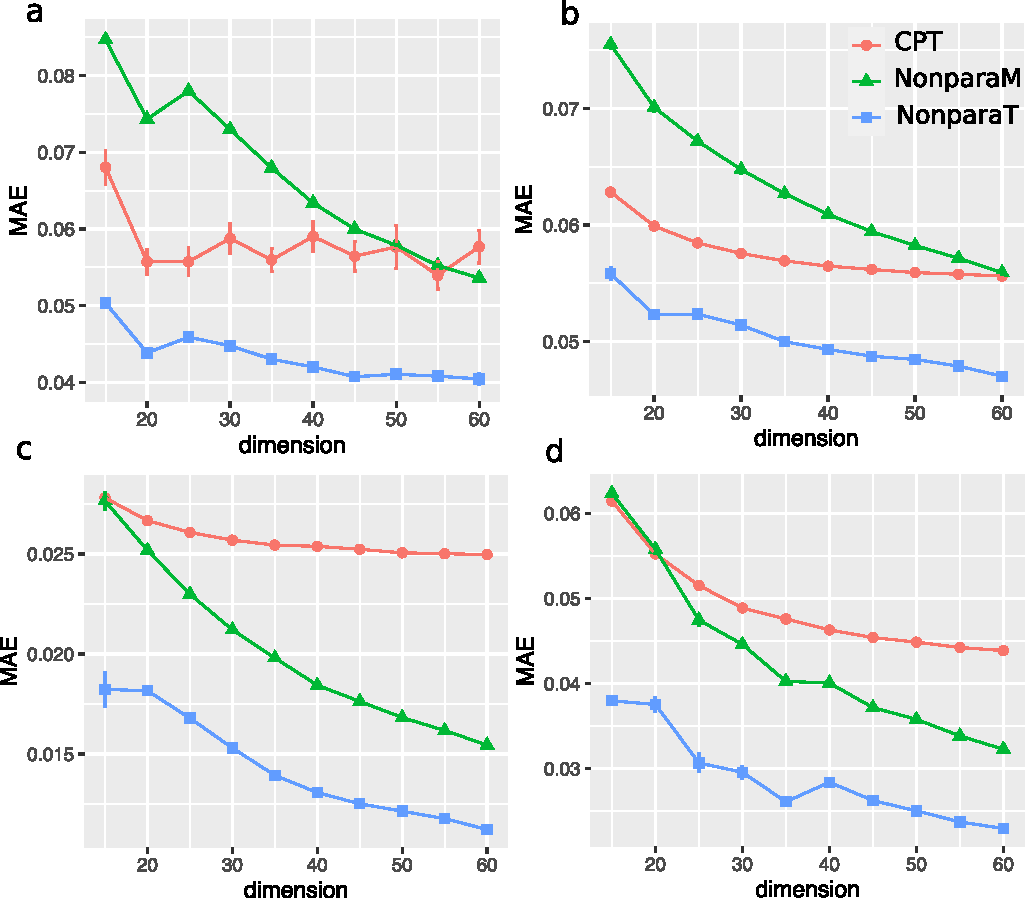
\includegraphics[width=.45\textwidth]{figure/fig1-4.pdf}
\vspace{-.4cm}
\caption{Estimation performance against tensor dimension. Panels (a)-(d) correspond to simulation models 1-4 in Table~\ref{tab:simulation}.}\label{fig:compare1}
\vspace{-.2cm}
\end{figure}


Figure~\ref{fig:compare1} compares the estimation error with full observation. We find all three methods show decreased error as the dimension increases. Furthermore, our method {\bf NonParaT} achieves the best performance in all scenarios, whereas the second best method is {\bf CPT} for models 1-2, and {\bf NonParaM} for models 3-4. One possible reason is that models 1-2 have controlled multilinear tensor rank, which makes tensor methods {\bf NonParaT} and {\bf CPT} more accurate than matrix methods. For models 3-4, the rank exceeds the tensor dimension, and the two nonparametric methods {\bf NonParaT} and {\bf NonparaM} are well suited for high rank signals. 

%The result also demonstrates the robustness of our method to various shapes of $\Theta(\omega)$. As we shown in Section~\ref{sec:identifiability}, the CDF of $\Theta(\omega)$ plays a key role in estimation accuracy, and a jump at $\pi$ makes $\pi$-weighted classification hard. Nevertheless, we find that our method maintains good performance in model 1 where the signal tensor $\Theta(\omega)$ has $3^3$ many jumps. The reason of this robustness is that we aggregate in total $(2H+1)$ sign tensors, each of which incurs at most ${1\over H}$ error to the final tensor estimate. Therefore, the estimation is robust against a few off-target sign tensor estimations, as long as the majority are accurate.  


Figure~\ref{fig:compare2} shows the completion error against observation fraction. We fix $d=40$ and gradually increase the observation fraction ${|\Omega|\over d^3}$ from 0.3 to 1. It is seen that our method achieves the lowest error among all methods. % Our simulation covers a reasonable range of various complexities, and the improved accuracy highlights the ability of our nonparametric method in tensor completion. 
We point out that the simulated models do not necessarily satisfy our method assumption. In particular, models 1 and 3 have unbounded noise, and model 2 has non-monotonic transformation functions. Nevertheless, our method shows good performance in spite of model misspecification. This result is appealing in practice because the structure of underlying signal tensor is often unknown. 

\begin{figure}[H]
\vspace{-.1cm}
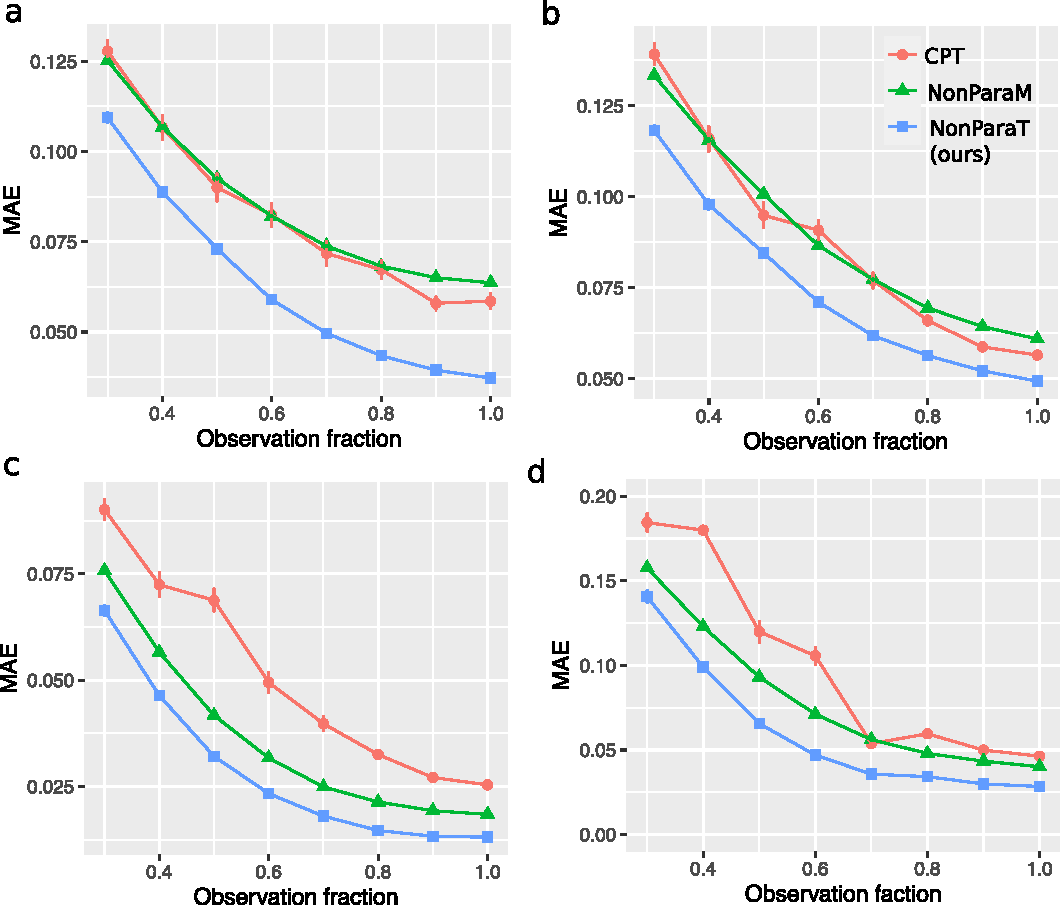
\includegraphics[width=.45\textwidth]{figure/fig5-8.pdf}
\caption{Completion performance against observation fraction. Panels (a)-(d) correspond to simulation models 1-4 in Table~\ref{tab:simulation}. }\label{fig:compare2}
\vspace{-.4cm}
\end{figure}

\section{Data analysis}
We apply our method to two tensor datasets, the MRN-114 human brain connectivity data~\citep{wang2017bayesian}, and NIPS data~\cite{globerson2007euclidean}. The MRN-144 dataset records the structural connectivity among 68 brain regions for 114 individuals along with their Intelligence Quotient (IQ) scores. We organize the connectivity data into an order-3 tensor, where entries encode the presence or absence of fiber connections between brain regions across individuals. The NIPS dataset consists of counts of words in NIPS papers published from 1987 to 2003. We focus on the top 100 authors, 200 most frequent words, and normalize each word count by log transformation with pseudocount 1. The resulting dataset is an order-3 tensor with entry representing the log counts of words by authors across years. 

Table~\ref{tab:data} compares the prediction accuracy of our method and low-rank CP method. The reported MAE is averaged over five runs of cross-validation, with 20\% entries for testing and 80\% for training. Our method substantially outperforms the classical low-rank method for every configuration in the considered range. Further increment of rank appears to have little effect on the performance, and we find that increased missingness gives more advantages to our method (see details in Appendix). In contrast, the low-rank CPT exhibits poor prediction even at a relatively high rank. The comparison highlights the advantage of our method in achieving accuracy while maintaining low complexity. 

\begin{table}[h!]
\resizebox{.48\textwidth}{!}{
\begin{tabular}{c|c|c|c}
\Xhline{2\arrayrulewidth}
\multicolumn{4}{c}{MRN-144 brain connectivity dataset}\\
\Xhline{2\arrayrulewidth}
Method                    & $r=6$ &  $r=9$&$r=12$\\
\hline
NonparaT (Ours)  & {\bf 0.14}(0.003) &  {\bf 0.12}(0.004)&{\bf 0.12}(0.007)\\
CPT  & 0.23(0.006)&0.22(0.004)&0.21(0.004)\\
 \Xhline{2\arrayrulewidth}
\multicolumn{4}{c}{NIPS dataset}\\
 \Xhline{2\arrayrulewidth}
Method                    & $r=6$& $r=9$&$r=12$\\
\hline
NonparaT (Ours)  & {\bf 0.16}(0.002)& {\bf 0.15}(0.001)&{\bf 0.14}(0.001)\\
CPT &0.20(0.007)&0.19(0.007)&0.17(0.007)
%Naive imputation &\multicolumn{2}{c}{0.32(.001)}
\end{tabular}
}
\vspace{-.2cm}
\caption{Comparison of prediction error in the MRN-114 and NIPS data analysis. For low-rank CPT, we use R function {\tt rTensor} with default hyperparameters, and for our method, we set $H = 20$.}\label{tab:data}
\vspace{-.3cm}
\end{table}


\begin{figure}[h!]
\centering
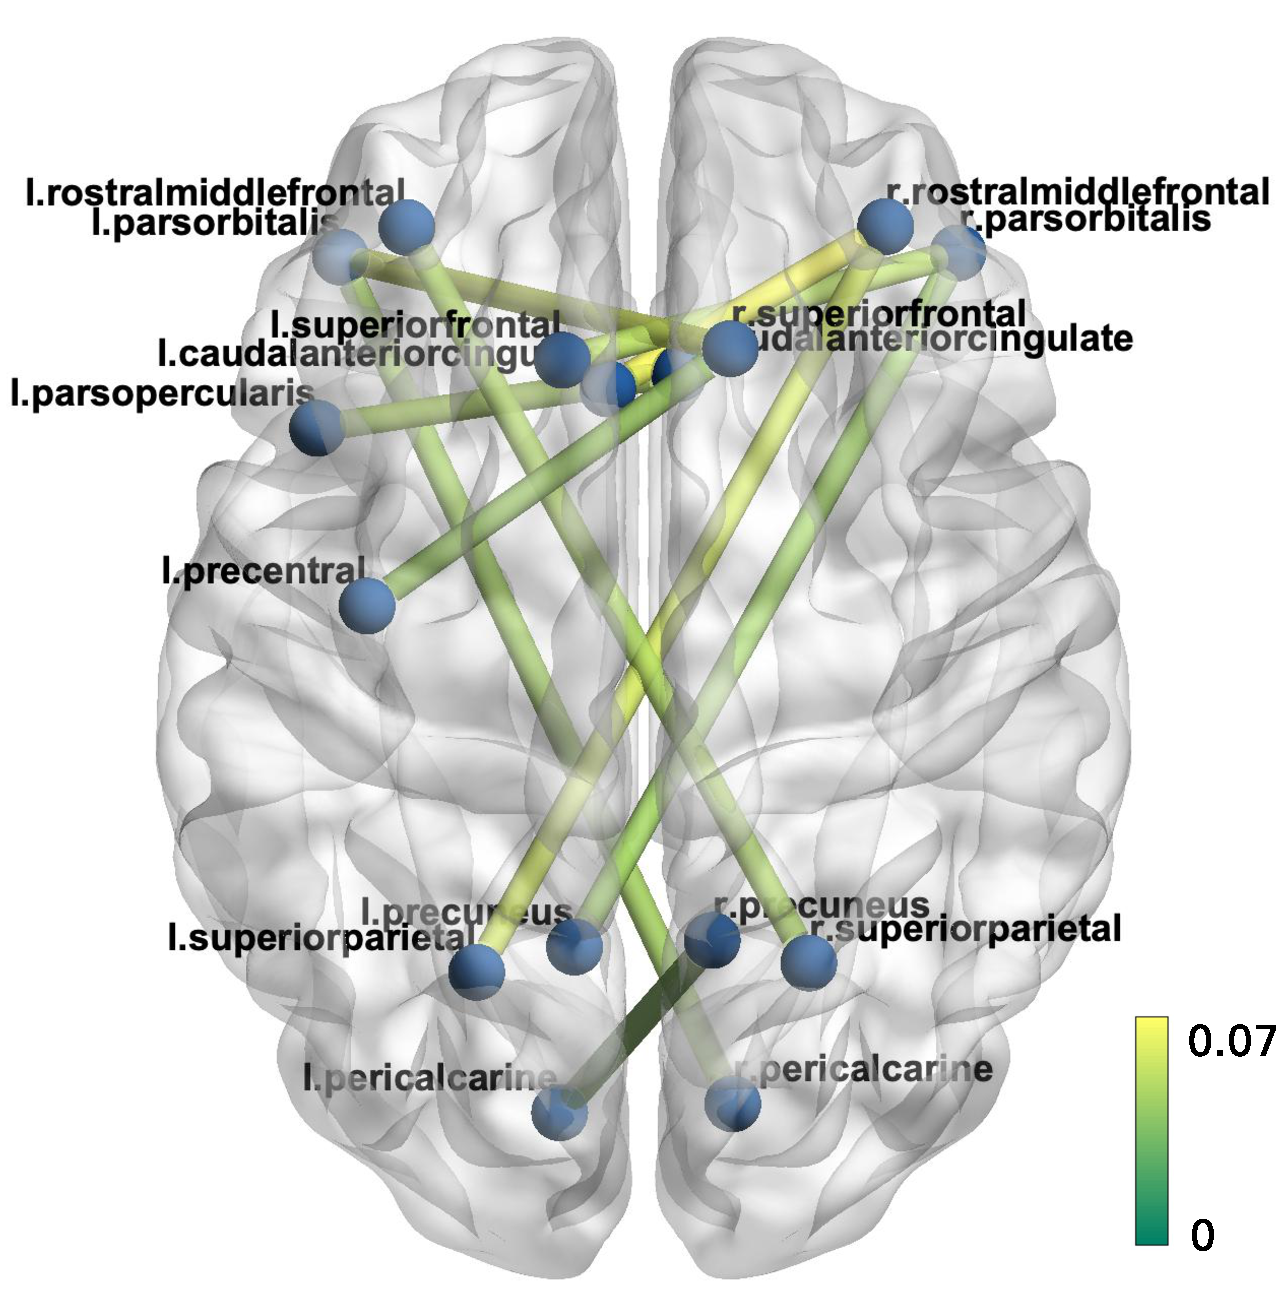
\includegraphics[width=.2\textwidth]{figure/brainIQ.pdf}
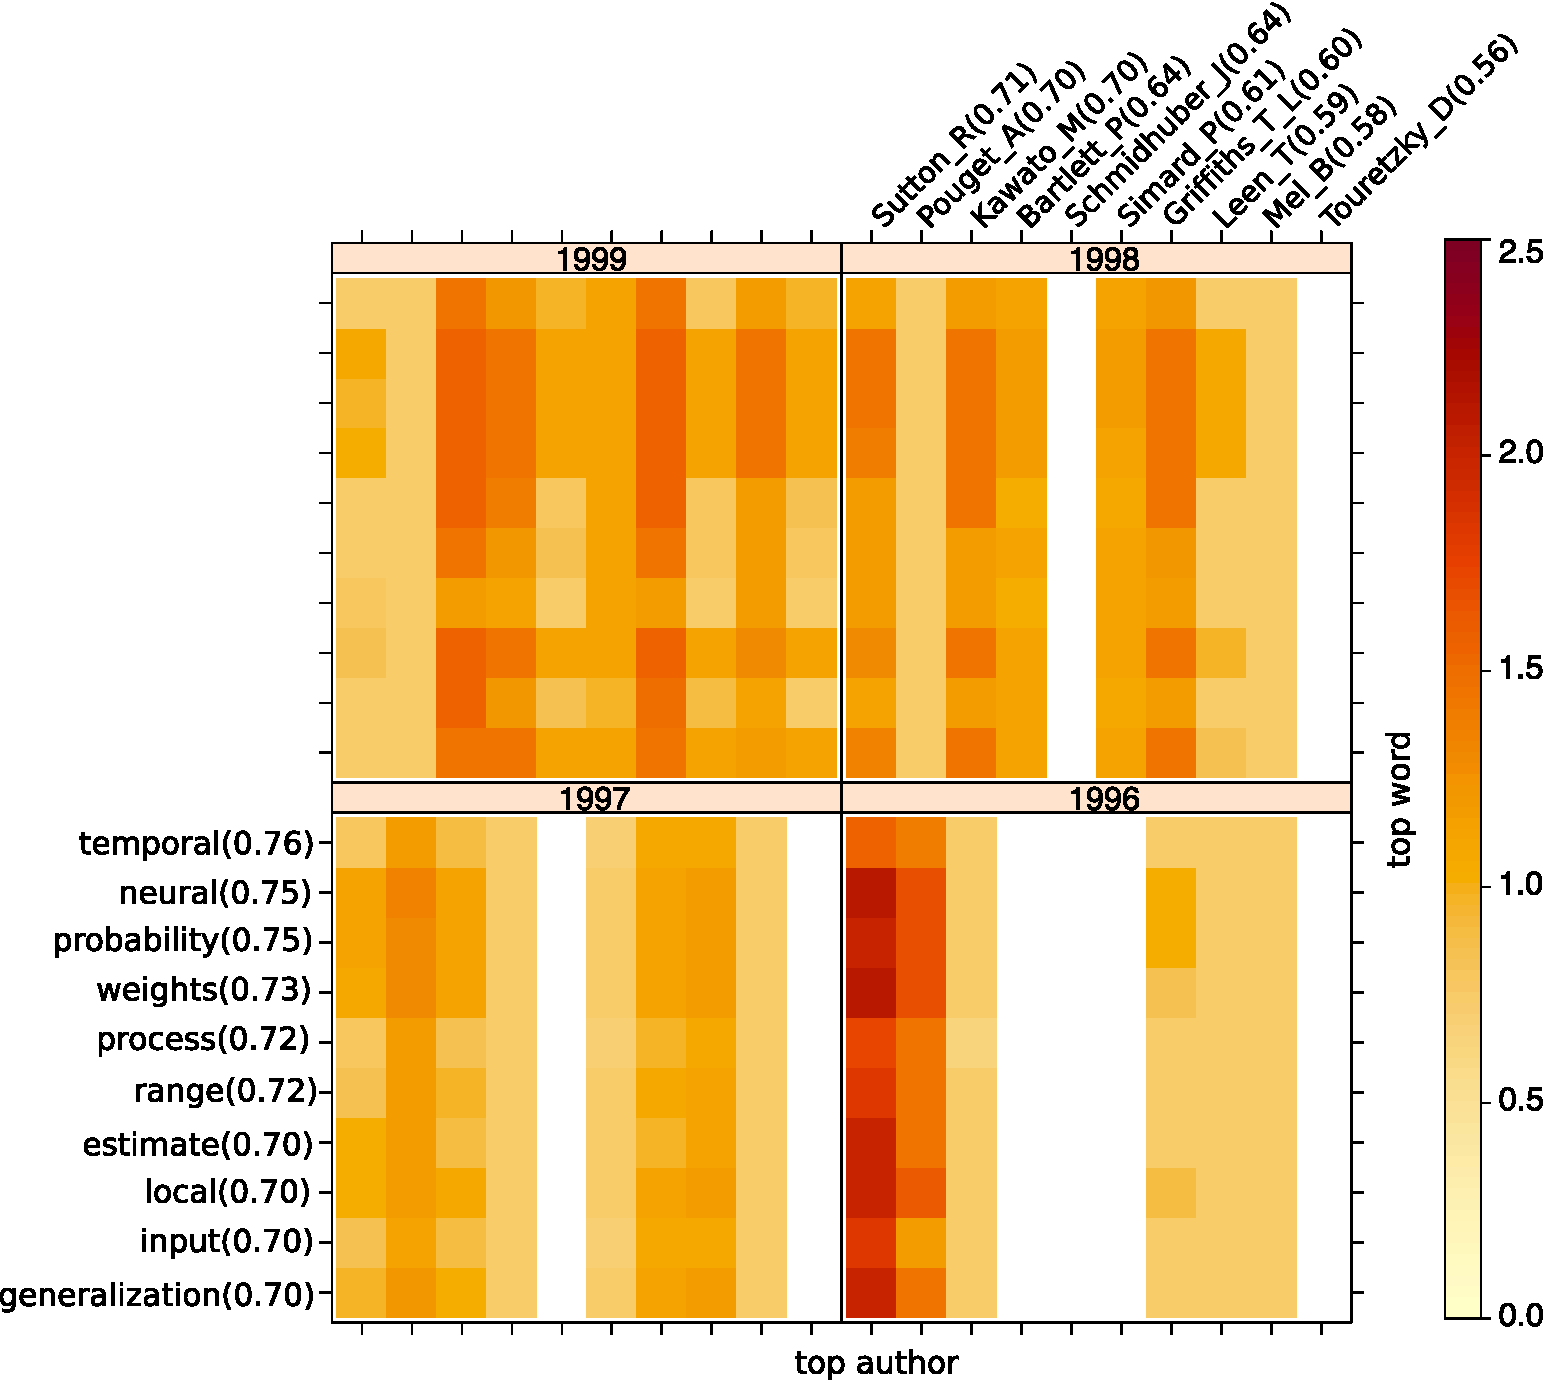
\includegraphics[width=.27\textwidth]{figure/signal.pdf}
\caption{Estimated signal tensor from brain connectivity data (a) and NIPS data (b). %Authors and words are ranked by marginal averages based on $\hat \Theta$, where the marginal average is denoted in the parentheses.
}\label{fig:signal}
\vspace{-.5cm}
\end{figure}

We next examine the estimated signal tensor $\hat \Theta$ form our method. Figure~\ref{fig:signal}a shows the top 10 edges in MSN-144 dataset based on regression analysis of denoised edge connection with IQ scores. We find that top edges are mostly inter-hemisphere, which are consistent with recent research in brain connectivity pattern with intelligence~\cite{li2009brain,wang2017bayesian}. Figure~\ref{fig:signal}b illustrates the result from NIPS data, where we plot the top entries in $\hat \Theta$ corresponding to top authors and words (after excluding generic words such as \emph{figure}, \emph{current}, etc). The detected patten is consistent with the active topics in the NIPS publication. Among the top words are \emph{temporal} (marginal mean = 0.76), \emph{neural} (0.75), and \emph{generalization} (0.70), whereas top authors are \emph{Richard Sutton} (0.71), \emph{Pouget\_A}(0.70), \emph{Kawato\_M} (0.70), and \emph{Bartlett Peter} (0.64). We also find strong heterogeneity among word occurrence across authors and years. For example, \emph{neural} and \emph{weights} are popular words for \emph{Tomas Griffiths} in 1998-1999, whereas \emph{temproal} occurs more often in \emph{Richard Sutton et al} in 1996. The achieved denoising accuracy and pattern detection demonstrates the applicability of our method.

\section{Conclusion}
We have develop a new framework for high rank tensor estimation based on sign tensor representations. Statistical accuracies are established, and we demonstrate the outperformance of our approach compared to other methods. The work unlocks several directions of future research. While we have provided numerical evidence for the success of nonconvex approach, the interplay be- tween computational efficiency and statistical accuracy remains an interesting future problem. 
\bibliographystyle{chicago}

\bibliography{tensor_wang}

\appendix

\end{document}
